%% LyX 2.3.6.1 created this file.  For more info, see http://www.lyx.org/.
%% Do not edit unless you really know what you are doing.
\documentclass[english]{article}
\usepackage[T1]{fontenc}
\usepackage[latin9]{inputenc}
\usepackage{geometry}
\geometry{verbose,tmargin=2.5cm,bmargin=2.5cm,lmargin=2.5cm,rmargin=2.5cm}
\usepackage{array}
\usepackage{amstext}
\usepackage{graphicx}
\PassOptionsToPackage{normalem}{ulem}
\usepackage{ulem}

\makeatletter

%%%%%%%%%%%%%%%%%%%%%%%%%%%%%% LyX specific LaTeX commands.
%% Because html converters don't know tabularnewline
\providecommand{\tabularnewline}{\\}

\makeatother

\usepackage{babel}
\begin{document}
{[}SPLIT\_HERE{]}
\begin{enumerate}
\item \textbf{{[}ALVL/9597/2017/P1/Q1{]} }

A role-playing computer game includes a list of items called the inventory.
This inventory can be represented using a one-dimensional (1 -D) array
or a list structure. 

\texttt{INVENTORY.TXT} is a text file containing the items from the
computer game inventory. Each item type can have many occurrences.
For example: 

\begin{tabular}{lll}
\textbf{Inventory} &  & \textbf{ItemType}\tabularnewline
Iron Ore &  & Iron Ore\tabularnewline
Stone &  & Stone\tabularnewline
Sticky Piston &  & Sticky Piston\tabularnewline
Glass &  & Glass \tabularnewline
Stone &  & Sand \tabularnewline
Stone &  & \tabularnewline
Sand &  & \tabularnewline
Sticky Piston &  & \tabularnewline
Iron Ore &  & \tabularnewline
\end{tabular}

\subsubsection*{Task 1.1}

Design and write program code to: 
\begin{itemize}
\item read the entire contents of \texttt{INVENTORY.TXT} to an appropriate
data structure called Inventory 
\item find each item type in this inventory and write these into a second
similar data structure called \texttt{ItemTypes} 
\item count the number of each item type in the inventory and store this
in a third similar data structure called \texttt{ItemCounts }
\item display the contents of the ItemTypes and ItemCounts data structures
using the format given below. 
\end{itemize}
Example run of the program: 

\begin{tabular}{lllll}
\textbf{Inventory} &  & \multicolumn{3}{l}{The output generated from this input would be:}\tabularnewline
Iron Ore &  &  &  & \tabularnewline
Stone &  & \textbf{ItemType} &  & \textbf{Count}\tabularnewline
Sticky Piston &  &  &  & \tabularnewline
Glass &  & Iron Ore &  & 2\tabularnewline
Stone &  & Stone &  & 3\tabularnewline
Stone &  & Sticky Piston &  & 2\tabularnewline
Sand &  & Glass &  & 1\tabularnewline
Sticky Piston &  & Sand &  & 1\tabularnewline
Iron Ore &  &  &  & \tabularnewline
\end{tabular}

\subsubsection*{Evidence 1}

Your program code.\hfill{}{[}14{]}

\subsubsection*{Evidence 2}

Screenshot of your output. \hfill{}{[}1{]}

{[}SPLIT\_HERE{]}
\item \textbf{{[}ALVL/9597/2017/P1/Q2{]} }

Every published book has an international Standard Book Number (ISBN).
This ISBN is a 9-digit number plus a check digit which is calculated
and added to the end of the number. A weighted-modulus method is used
to calculate the check digit. 

This method uses a weighted modulus 11. If the check digit is calculated
as 10. it is replaced with the character 'X'. Where the check digit
is calculated as 11, it will be replaced with 0. 

\noindent %
\begin{tabular}{l}
184146208 will be calculated as\tabularnewline
$1\times10=10$\tabularnewline
$8\times9=72$\tabularnewline
$4\times8=32$\tabularnewline
$1\times7=7$\tabularnewline
$4\times6=24$\tabularnewline
$6\times5=30$\tabularnewline
$2\times4=8$\tabularnewline
$0\times3=0$\tabularnewline
$8\times2=16$\tabularnewline
Total = 199\tabularnewline
$199/11=18$ remainder 1\tabularnewline
$11-1=10$\tabularnewline
Therefore, 10 is replaced with X:\tabularnewline
ISBN is 184146208\textbf{X}\tabularnewline
\end{tabular}%
\begin{tabular}{l}
034085045 will be calculated as\tabularnewline
$0\times10=0$\tabularnewline
$7\times9=63$\tabularnewline
$5\times8=40$\tabularnewline
$1\times7=7$\tabularnewline
$5\times6=30$\tabularnewline
$4\times5=20$\tabularnewline
$9\times4=36$\tabularnewline
$2\times3=6$\tabularnewline
$6\times2=12$\tabularnewline
Total = 154\tabularnewline
$154/11=14$ remainder 0\tabularnewline
$11-0=11$\tabularnewline
Therefore, 11 is replaced with 0:\tabularnewline
ISBN is 034085045\textbf{0}\tabularnewline
\end{tabular}%
\begin{tabular}{l}
075154926 will be calculated as\tabularnewline
$0\times10=0$\tabularnewline
$3\times9=27$\tabularnewline
$4\times8=32$\tabularnewline
$0\times7=0$\tabularnewline
$8\times6=48$\tabularnewline
$5\times5=25$\tabularnewline
$0\times4=0$\tabularnewline
$4\times3=12$\tabularnewline
$5\times2=10$\tabularnewline
Total = 214\tabularnewline
$214/11=19$ remainder 5\tabularnewline
$11-5=6$\tabularnewline
Therefore, 6 is added to the\tabularnewline
end of the ISBN: 075154926\textbf{6} \tabularnewline
\end{tabular}

\subsubsection*{Task 2.1}

Study the identifier table and the incomplete recursive algorithm
on the opposite page. 

The missing lines in the algorithm are labelled \textbf{A}, \textbf{B}
and \textbf{C}. 

Write the\textbf{ three} missing lines of code. Label each as \textbf{A},
\textbf{B} or \textbf{C}. \hfill{} {[}3{]}

\subsubsection*{Evidence 3}

The three missing lines of code. \hfill{}{[}3{]}
\begin{center}
\begin{tabular}{|l|c|l|}
\hline 
\textbf{Identifier} & \textbf{Data Type} & \textbf{Description}\tabularnewline
\hline 
\texttt{Number} & \texttt{STRING} & The ISBN to be processed\tabularnewline
\hline 
\texttt{Digit} & \texttt{lNTEGER} & A digit from the iSBN to be processed\tabularnewline
\hline 
\texttt{Total} & \texttt{INTEGER} & Running total for modulus calculation\tabularnewline
\hline 
\texttt{NewNumber} & \texttt{STRING} & A version of the list string shortened by removing the first character\tabularnewline
\hline 
\texttt{CheckDigit} & \texttt{STRING} & The calculated check digit value\tabularnewline
\hline 
\texttt{CalcModulus} & \texttt{INTEGER} & Used to store the result of \texttt{(Total MOD 11)}\tabularnewline
\hline 
\texttt{CheckValue} & \texttt{INTEGER} & Used to store the result of \texttt{(11 - CalcModulus)}\tabularnewline
\hline 
\end{tabular}
\par\end{center}

\noindent %
\noindent\begin{minipage}[t]{1\columnwidth}%
\texttt{FUNCTION CalCheckDigit(Number AS STRING, Total AS INTEGER)
RETURNS STRING }

\texttt{\qquad{}IF LENGTH(Number) > 1 THEN }

\texttt{\qquad{}\qquad{}Digit <- INTEGER(LEFT(Number,1)) }

\texttt{\qquad{}\qquad{}Total <- Total + (Digit {*} (LENGTH(Number)+1)) }

\texttt{\qquad{}\qquad{}NewNumber <- RIGHT(Number, LENGTH(Number)-1) }

\texttt{\qquad{}\qquad{}CheckDigit <- .................. A ................. }

\texttt{\qquad{}ELSE }

\texttt{\qquad{}\qquad{}Digit <- INTEGER(LEFT(Number,1)) }

\texttt{\qquad{}\qquad{}Total <- Total + (Digit 1 (LENGTH(Number)+1)) }

\texttt{\qquad{}\qquad{}CalcModulus <- Total MOD 11 }

\texttt{\qquad{}\qquad{}CheckValue <- 11 - CalcModulus }

\texttt{\qquad{}\qquad{}IF CheckValue = 11 THEN }

\texttt{\qquad{}\qquad{}\qquad{}RETURN STRING(O) }

\texttt{\qquad{}\qquad{}ELSE }

\texttt{\qquad{}\qquad{}\qquad{}IF CheckValue = 10 THEN }

\texttt{\qquad{}\qquad{}\qquad{}....................... B .......................... }

\texttt{\qquad{}\qquad{}\qquad{}ELSE }

\texttt{\qquad{}\qquad{}\qquad{}RETURN STRING(CheckValue) }

\texttt{\qquad{}\qquad{}\qquad{}ENDIF }

\texttt{\qquad{}\qquad{}ENDIF }

\texttt{\qquad{}ENDIF }

\texttt{\qquad{}IF LENGTH(Number) = 9 THEN }

\texttt{\qquad{}\qquad{}RETURN .................... C .................... }

\texttt{\qquad{}ELSE }

\texttt{\qquad{}\qquad{}RETURN CheckDigit; }

\texttt{\qquad{}ENDIF }

\texttt{END FUNCTION}

\bigskip{}

\texttt{// Calculate ISBN, an example of how the function is called. }

\texttt{// Second parameter is always 0. }

\texttt{ISBN = CalCheckDigit(\textquotedbl 184146208\textquotedbl ,0)}%
\end{minipage}

\subsubsection*{Task 2.2}

Write a program to implement the ISBN program using the \texttt{CalCheckDigit}
function.

The program will:
\begin{itemize}
\item read the entire contents of the file \texttt{ISBNPRE.TXT} (seven 9-digit
lSBNs without check digits) into an appropriate data structure
\item use the function \texttt{CalCheckDigit} to calculate the result (ISBN
with check digit) for each entry in the file
\item write each result (ISBN with check digit) to the screen.
\end{itemize}

\subsubsection*{Evidence 4}

Your program code for Task 2.2. \hfill{}{[}11{]}

\subsubsection*{Evidence 5}

Screenshot of the results of processing the \texttt{ISBNPRE.TXT} file.\hfill{}{[}1{]}

{[}SPLIT\_HERE{]}
\item \textbf{{[}ALVL/9597/2017/P1/Q3{]} }

A data structure is required to store 25 nodes. A linked list is maintained
of all the nodes. A node contains a data value and two pointers: a
left pointer and a right pointer. 

Items in the list are initially linked using their \texttt{LeftChild}
pointers. 

Each node ls implemented as an instance of the class \texttt{ConnectionNode}.
The class ConnectionNode has the following properties: 
\begin{center}
\begin{tabular}{|l|l|l|}
\hline 
\multicolumn{3}{|c|}{\texttt{Class: Connection Node}}\tabularnewline
\hline 
\multicolumn{3}{|c|}{Attributes}\tabularnewline
\hline 
\texttt{\hspace{0.01\columnwidth}}Identifier & \texttt{\hspace{0.01\columnwidth}}Data Type & \texttt{\hspace{0.05\columnwidth}}Description\tabularnewline
\hline 
\texttt{DataValue} & \texttt{STRING} & The node data\tabularnewline
\hline 
\texttt{LeftChild} & \texttt{INTEGER} & The left node pointer \tabularnewline
\hline 
\texttt{RightChild} & \texttt{INTEGER} & The right node pointer\tabularnewline
\hline 
\end{tabular}
\par\end{center}

The structure for the linked list is implemented as follows: 
\begin{center}
\begin{tabular}{|l|c|l|}
\hline 
\texttt{\hspace{0.01\columnwidth}}Identifier & Data Type & \texttt{\hspace{0.05\columnwidth}}Description\tabularnewline
\hline 
\texttt{RobotData} & \texttt{ARRAY {[}l : 25{]} OF ConnectionNode} & An array used to store the\tabularnewline
 &  & 25 nodes.\tabularnewline
\hline 
\texttt{Root} & \texttt{INTEGER} & Index for the root position \tabularnewline
 &  & of the \texttt{RobotData} array\tabularnewline
\hline 
\texttt{NextFreeChild} & \texttt{INTEGER} & Index for the next \tabularnewline
 &  & available empty node\tabularnewline
\hline 
\end{tabular}
\par\end{center}

The first available node Is indicated by \texttt{NextFreeChild}. The
initial value of \texttt{Root} is 1 and the initial value of \texttt{NextFreeChild}
is 1.

The diagram shows the empty data structure with the linked list to
record the unused nodes. 
\begin{center}
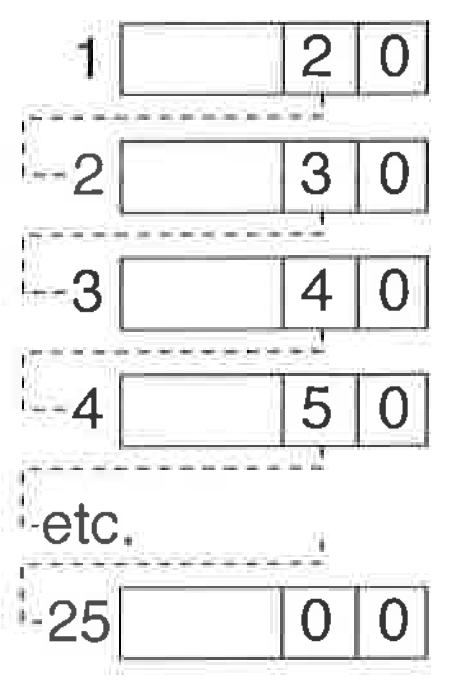
\includegraphics[width=0.125\paperwidth]{C:/Users/Admin/Desktop/Github/question_bank/LyX/static/img/9597-ALVL-2017-P1-Q3-1}
\par\end{center}

\subsubsection*{Task 3.1}

Write the program code to declare the \textbf{empty} data structure
and linked list of 25 unused nodes. Add statement(s) to initiallse
the empty data structure.

\subsubsection*{Evidence 6}

Your program code for Task 3.1. \hfill{}{[}12{]}

This data structure is used to record the possible routes for a robot
to travel from a node A to a node Z. The following data structure
illustrates many possible routes, for example, A$\rightarrow$D$\rightarrow$K$\rightarrow$L$\rightarrow$M$\rightarrow$Z.
It is only possible to move to one of two possible nodes; for example,
from node A, the only move is to node B or node D.
\begin{center}
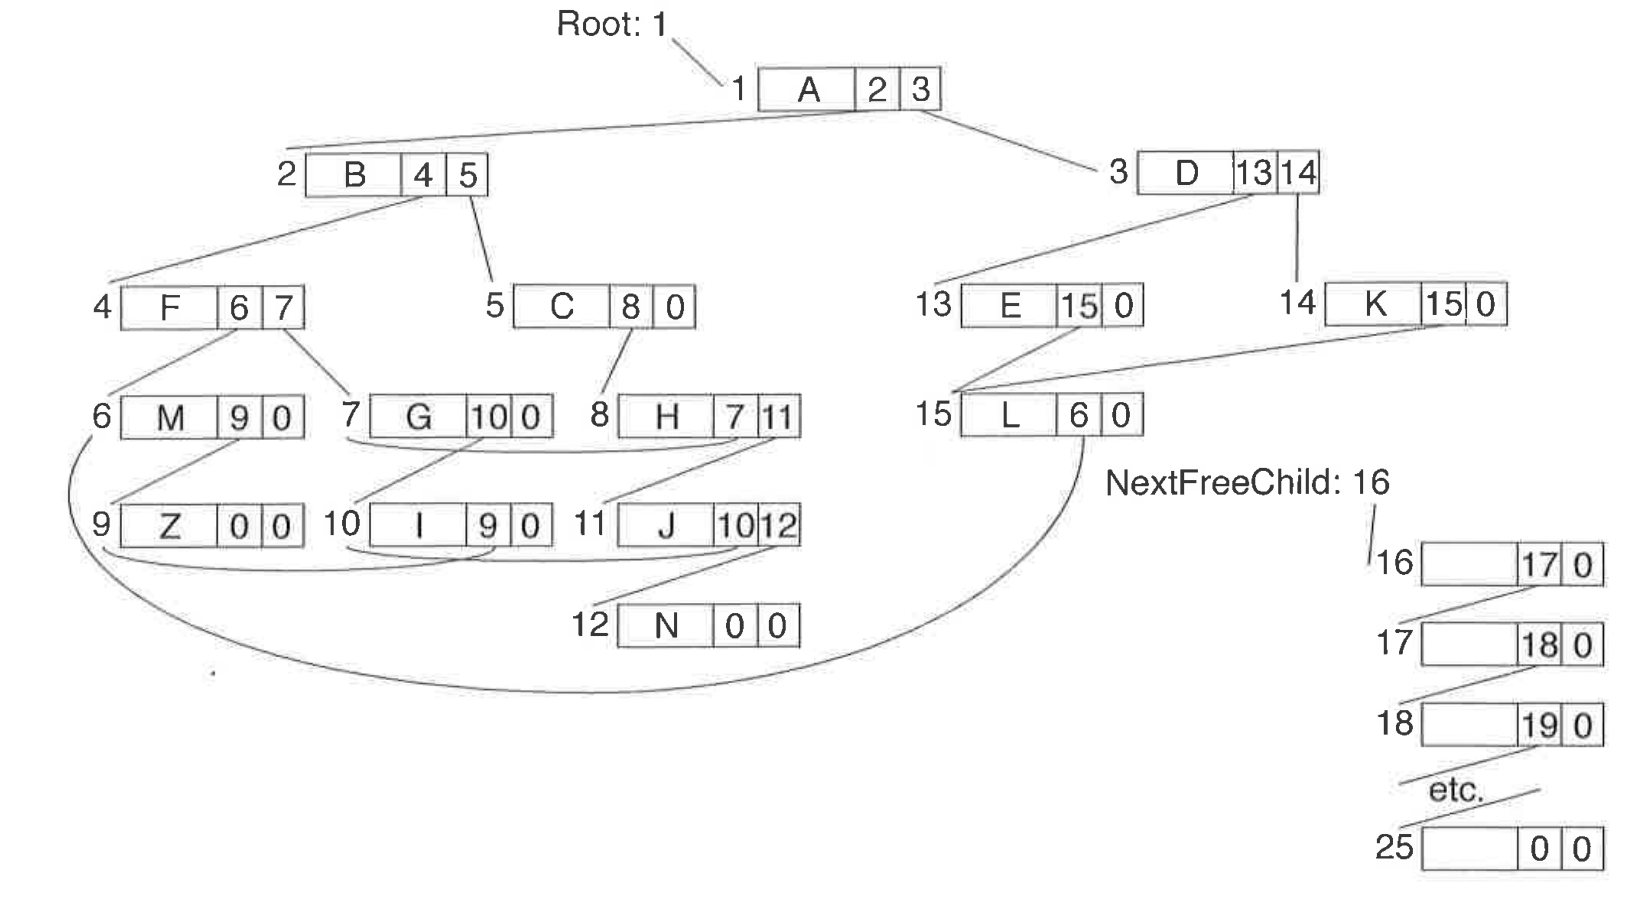
\includegraphics[width=0.5\paperwidth]{C:/Users/Admin/Desktop/Github/question_bank/LyX/static/img/9597-ALVL-2017-P1-Q3-2}
\par\end{center}

This data structure has 15 nodes (A to N and Z) but for future development
a maximum of 25 nodes is specified. All nodes are unique.

The pseudocode on the next page can be used to add a node to the data
structure. The procedure \texttt{AddToRobotData} uses the parameters
\texttt{NewDataItem}, \texttt{ParentItem} and \texttt{ThisMove}.

The parameter \texttt{ThisMove} holds the move made to create this
new item (\textquoteleft L' for LeftChild, \textquoteleft R' for RightChild,
\textquoteleft X\textquoteright{} for initial state/root), and the
\texttt{ParentItem} parameter holds the value of the parent item which
points to this \texttt{NewDataItem}.
\begin{center}
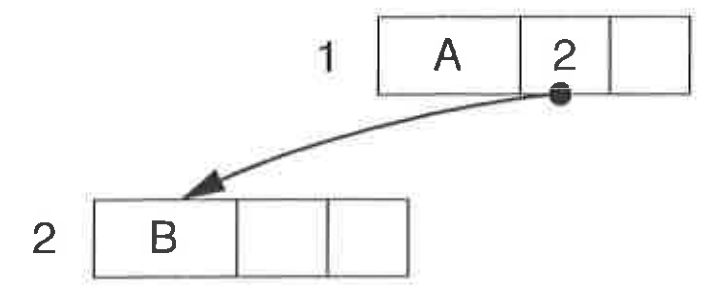
\includegraphics[width=0.25\paperwidth]{C:/Users/Admin/Desktop/Github/question_bank/LyX/static/img/9597-ALVL-2017-P1-Q3-3}
\par\end{center}

To add node B as shown, the procedure call would be \texttt{AddToRobotData
('B', \textquoteleft A', 'L')} . The parameters used would be: 

\texttt{B}, the new node 

\texttt{A}, the parent node 

\texttt{L}, the location of the child (which has an index of 2) is
recorded in \texttt{LeftChild} of A.

The following pseudocode (available in PS EUDOCODE\_TASK\_3\_2 . TXT)
can be used to add a node to the data structure.

\noindent %
\noindent\begin{minipage}[t]{1\columnwidth}%
\texttt{FUNCTION FindNode(NodeValue) RETURNS INTEGER }

\texttt{\qquad{}Found <- FALSE}

\texttt{\qquad{}CurrentPosition <- Root }

\texttt{\qquad{}REPEAT }

\texttt{\qquad{}\qquad{}IF RobotData{[}CurrentPosition{]}.DataValue
= NodeValue THEN }

\texttt{\qquad{}\qquad{}\qquad{}Found <- TRUE }

\texttt{\qquad{}\qquad{}ELSE }

\texttt{\qquad{}\qquad{}\qquad{}CurrentPosition <- CurrentPosition
+ 1 }

\texttt{\qquad{}\qquad{}ENDIF }

\texttt{\qquad{}UNTIL Found = TRUE OR CurrentPosition > 25 }

\texttt{\qquad{}IF CurrentPOSition > 25 THEN }

\texttt{\qquad{}\qquad{}RETURN 0}

\texttt{\qquad{}ELSE }

\texttt{\qquad{}\qquad{}RETURN CurrentPosition }

\texttt{\qquad{}ENDIF }

\texttt{ENDFUNCTION}

\bigskip{}

\texttt{PROCEDURE AddToRobotData(NewDataItem, ParentItem, ThisMove) }

\texttt{\qquad{}\qquad{}IF Root = 1 AND NextFreeChild = 1 THEN }

\texttt{\qquad{}\qquad{}\qquad{}NextFreeChild <- RobocData{[}NextFreeChild{]}.LeftChild }

\texttt{\qquad{}\qquad{}\qquad{}RobotDataIRoot{]}.LeftChild <-
0 }

\texttt{\qquad{}\qquad{}\qquad{}RobotData{[}Root{]}.DataValue <-
NewDataItem }

\texttt{\qquad{}\qquad{}ELSE }

\texttt{\qquad{}\qquad{}\qquad{}// does the parent exist? . }

\texttt{\qquad{}\qquad{}\qquad{}ParentPosition <- FindNode(ParentItem) }

\texttt{\qquad{}\qquad{}\qquad{}IF RarentPosition > 0 THEN // parent
exists }

\texttt{\qquad{}\qquad{}\qquad{}\qquad{}// does the child exist? }

\texttt{\qquad{}\qquad{}\qquad{}\qquad{}ExistingChild <- FindNode(NewDataItem)
' }

\texttt{\qquad{}\qquad{}\qquad{}\qquad{}IF ExistingChild > 0 THEN
// child exists }

\texttt{\qquad{}\qquad{}\qquad{}\qquad{}\qquad{}ChildPointer
<- ExistingChild }

\texttt{\qquad{}\qquad{}\qquad{}\qquad{}ELSE }

\texttt{\qquad{}\qquad{}\qquad{}\qquad{}ChildPointer <- NextFreeChild }

\texttt{\qquad{}\qquad{}\qquad{}\qquad{}NextFreeChild <- RobotDataINextFreeChild\}.LeftChild }

\texttt{\qquad{}\qquad{}\qquad{}\qquad{}RobotData{[}ChildPointer{]}.LeftChild
<- 0 }

\texttt{\qquad{}\qquad{}\qquad{}\qquad{}RobotData{[}ChildPointer{]}.DataValue
<- NewDataItem }

\texttt{\qquad{}\qquad{}\qquad{}\qquad{}ENDIF }

\texttt{\qquad{}\qquad{}\qquad{}\qquad{}IF ThisMove = 'L' THEN }

\texttt{\qquad{}\qquad{}\qquad{}\qquad{}\qquad{}RobotData{[}ParentPosition{]}.LeftChild
<- ChildPointer }

\texttt{\qquad{}\qquad{}\qquad{}\qquad{}ELSE }

\texttt{\qquad{}\qquad{}\qquad{}\qquad{}\qquad{}RobotData{[}ParentPosition{]}.RightChild
<- ChildPointer }

\texttt{\qquad{}\qquad{}\qquad{}\qquad{}ENDIF }

\texttt{\qquad{}\qquad{}\qquad{}ENDIF}\textbf{ }

\texttt{\qquad{}\qquad{}ENDIF }

\texttt{ENDPROCEDURE}%
\end{minipage}

\subsubsection*{Task 3.2}

Write code to implement \texttt{AddToRobotData} and \texttt{FindNode}
from this pseudocode.

You may use the text file \texttt{PSEUDOCODE\_TASK\_3\_2.TXT} as a
basis for writing your code.

\subsubsection*{Evidence 7}

Your program code for Task 3.2. \hfill{}{[}7{]}

\subsubsection*{Task 3.3}

Write a procedure \texttt{OutputData} which displays the value of
\texttt{Root}, the value of \texttt{NextFreeChild} and the contents
of \texttt{RobotData} in index order.

\subsubsection*{Evidence 8}

Your program code for Task 3.3.\hfill{} {[}6{]}

\subsubsection*{Task 3.4}

The file \texttt{SEARCHTREE.TXT} contains the data for the search
tree. Each row of the file contains three comma separated values,
for example, the first row contains '\texttt{A}', '\texttt{0}' and
'X'. The file is organised as: \texttt{NewDataltem, ParentItem, ThisMove}

\texttt{NewDataItem, ParentItem, ThisMove}

\texttt{$\dots$}

\texttt{<End of File>}

There are a total of 20 lines in the \texttt{SEARCHTREE.TXT} file
representing possible routes.

Write a main program to read the contents of this file and use \texttt{AddToRobotData}
and \texttt{FindNode} to insert these routes into \texttt{RobotData}.
Your program will then call the \texttt{OutputData} procedure. 

\subsubsection*{Evidence 9}

Your program code for Task 3.4. \hfill{}{[}6{]}

\subsubsection*{Evidence 10}

Screenshot showing the output from running the program in Task 3.4.\hfill{}
{[}2{]}

\subsubsection*{Task 3.5}

Write a recursive pre-order tree traversal that will display all valid
routes from A to Z by following the routes described in \texttt{RobotData}.

\subsubsection*{Evidence 11}

Your program code for Task 3.5.\hfill{} {[}6{]}

\subsubsection*{Evidence 12}

Screenshot showing the output from running the program in Task 3.5.\hfill{}
{[}1{]}

{[}SPLIT\_HERE{]}
\item \textbf{{[}ALVL/9597/2017/P1/Q4{]} }

A computer program can generate a simple Sudoku puzzle using a 4 x
4 two-dimensional array. 

An example of this puzzle is: 
\begin{center}
\begin{tabular}{|c|c|c|c|}
\hline 
4 & 3 & 2 & 1\tabularnewline
\hline 
1 & 2 & 4 & 3\tabularnewline
\hline 
3 & 4 & 1 & 2\tabularnewline
\hline 
2 & 1 & 3 & 4\tabularnewline
\hline 
\end{tabular}
\par\end{center}

The first step to creating this puzzle is to develop a program to
display the 4 x 4 twodimensional array as a grid. This program will
display the grid as: 
\begin{center}
\begin{tabular}{cccc}
4 & 3 & 2 & 1\tabularnewline
1 & 2 & 4 & 3\tabularnewline
3 & 4 & 1 & 2\tabularnewline
2 & 1 & 3 & 4\tabularnewline
\end{tabular}
\par\end{center}

\subsubsection*{Task 4.1}

Create a program design that will declare, initialise and display
the example puzzle shown. This design will: 
\begin{itemize}
\item make use of top-down design 
\item include the data structure to represent the puzzle as a grid 
\item initialise the grid using the values shown
\item make use of appropriate procedures and/or functions. 
\end{itemize}

\subsubsection*{Evidence 13}

Your program design for Task 4.1. \hfill{}{[}6{]}

\subsubsection*{Task 4.2}

Write program code to display the puzzle designed in Task 4.1. 

\subsubsection*{Evidence 14}

Your program code.\hfill{} {[}5{]}

\subsubsection*{Evidence 15}

Screenshot of the displayed grid. \hfill{}{[}1{]}

The puzzle is said to be valid if it follows these rules:
\begin{itemize}
\item It consists of tour quadrants.
\item The numbers in each quadrant must add up to ten.
\item Each horizontal and vertical row of the puzzle must also add up to
ten.
\item No number can be repeated in the same row, same column or same quadrant
of the puzzle. 
\end{itemize}
A good strategy tor creating puzzles is to start with a valid \textquoteleft base'
puzzle and perform transformations on it to create new puzzles.

You will write program code to create new valid puzzles. 

Each puzzle created will have two randomly selected transformations.
from a possible four, performed on it. The following are the four
possible transformations that can be carried out. 
\begin{center}
\begin{tabular}{|c|>{\raggedright}p{0.3\columnwidth}|l|}
\hline 
\textbf{Transformation} & \texttt{\hspace{0.05\columnwidth}}Explanation & \multicolumn{1}{l}{}\tabularnewline
\hline 
\textbf{1} & Swaps two rows in the same quadrants & \tabularnewline
 &  & 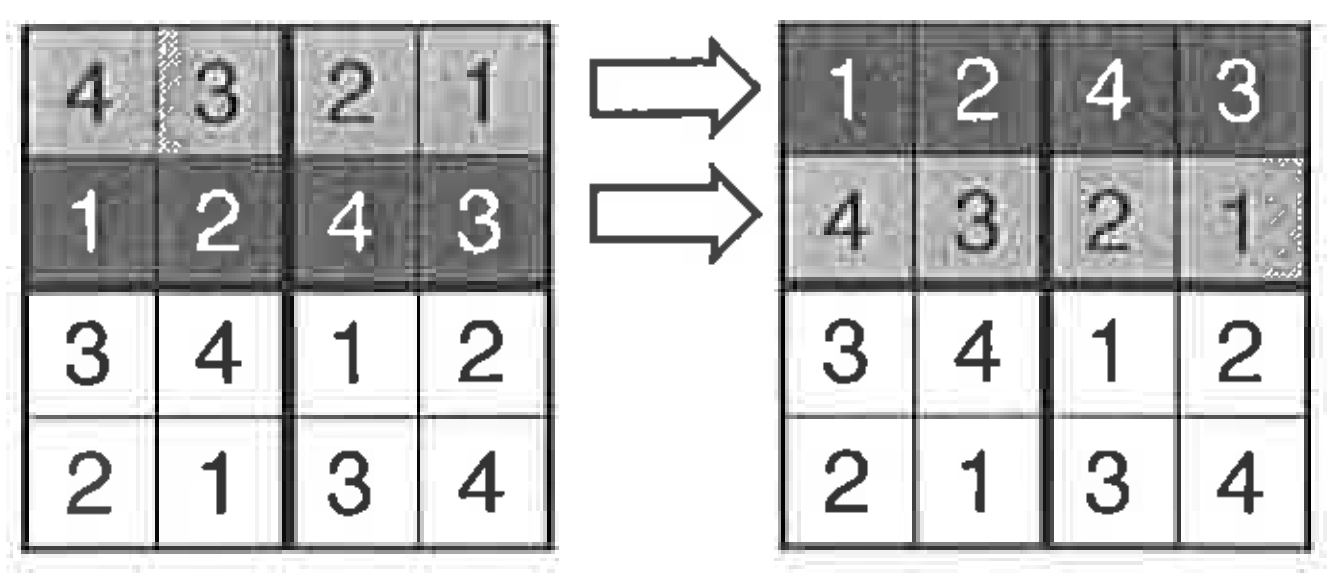
\includegraphics[width=0.3\paperwidth]{C:/Users/Admin/Desktop/Github/question_bank/LyX/static/img/9597-ALVL-2017-P1-Q4-1}\tabularnewline
\hline 
\textbf{2} & Swaps two columns in the same quadrants & \tabularnewline
 &  & 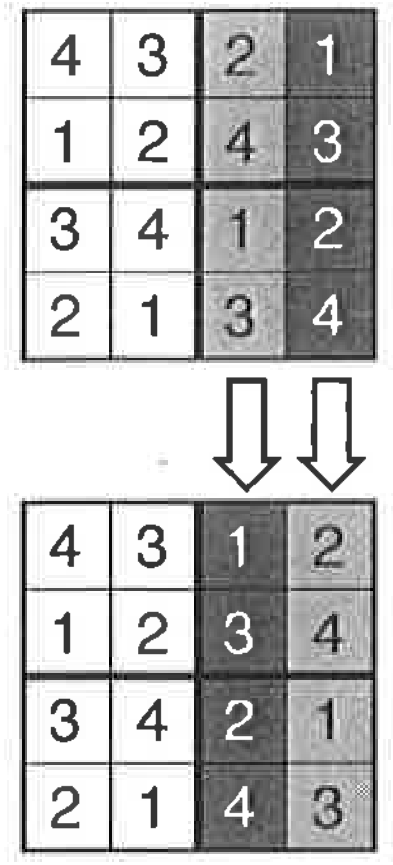
\includegraphics[width=0.15\paperwidth]{C:/Users/Admin/Desktop/Github/question_bank/LyX/static/img/9597-ALVL-2017-P1-Q4-2}\tabularnewline
\hline 
\textbf{3} & Swaps the top and bottom quadrant rows entirely & \tabularnewline
 &  & 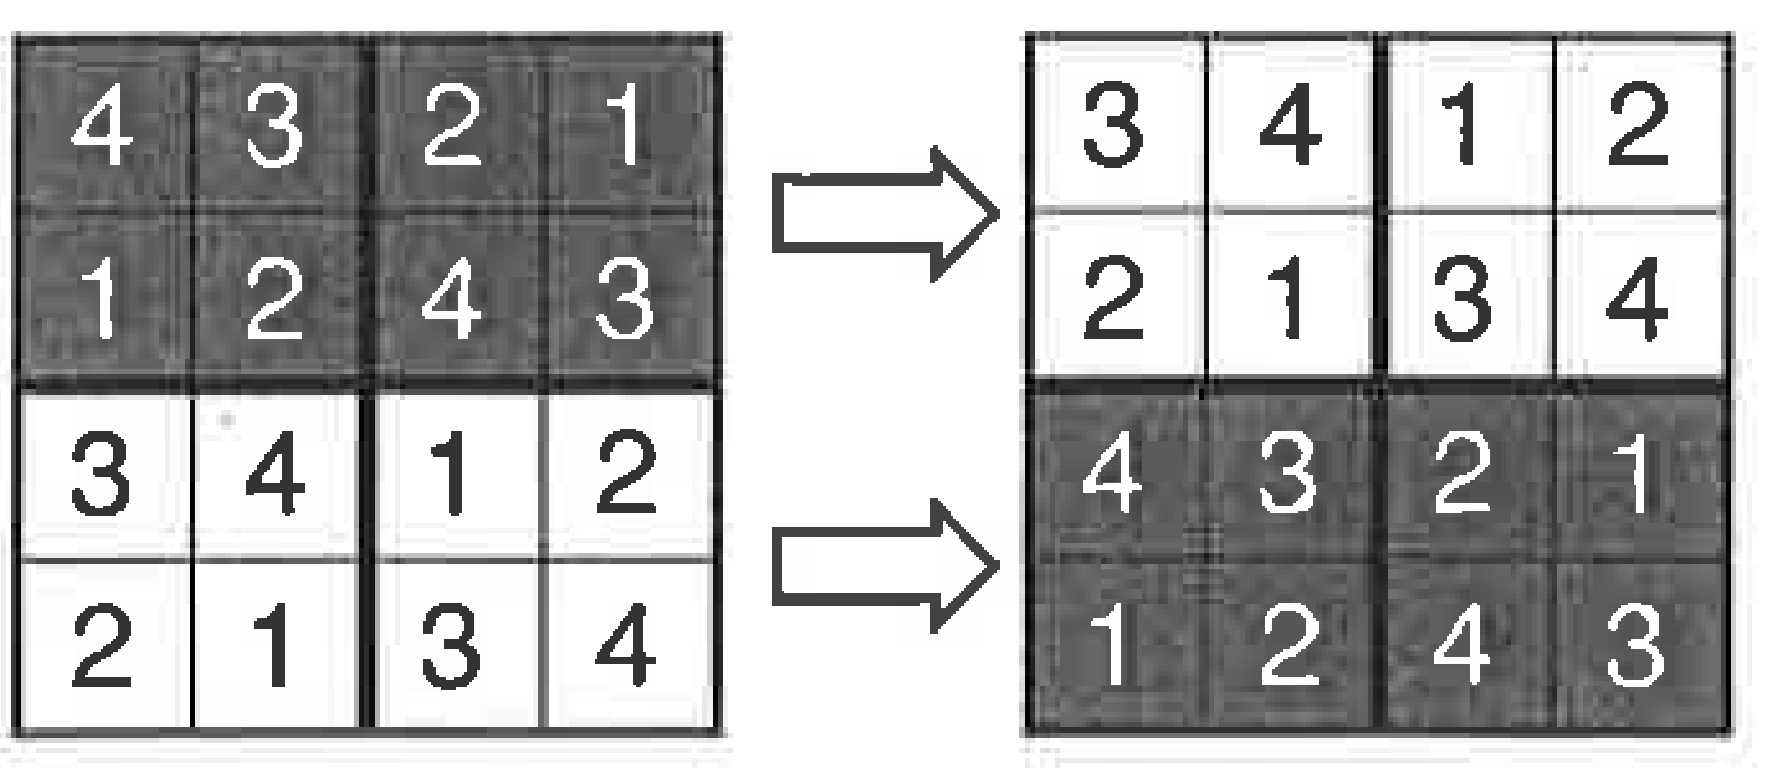
\includegraphics[width=0.3\paperwidth]{C:/Users/Admin/Desktop/Github/question_bank/LyX/static/img/9597-ALVL-2017-P1-Q4-3}\tabularnewline
\hline 
\textbf{4} & Swaps the left and right quadrant columns entirely & \tabularnewline
 &  & 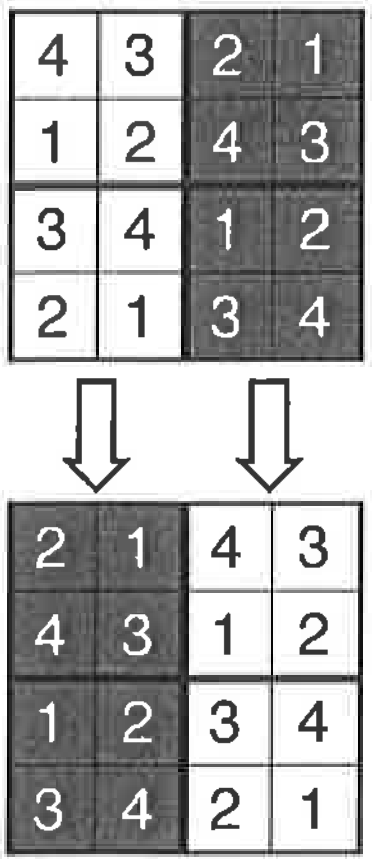
\includegraphics[width=0.15\paperwidth]{C:/Users/Admin/Desktop/Github/question_bank/LyX/static/img/9597-ALVL-2017-P1-Q4-4}\tabularnewline
\hline 
\end{tabular}
\par\end{center}

\subsubsection*{Task 4.3}

Write additional program code with brief \textbf{internal commentary}
to identify each transformation. 

The program code will: 
\begin{itemize}
\item create a method of selecting. at random, two of the four possible
transformations to be applied to the puzzle 
\item call a sub-program for each of the required transformations 
\item randomly select which rows will be transformed for transformations
1 and 2. for example. either the top or bottom two rows (for transformation
1) OR either the left-most or right-most two columns (for transformation
2) respectively 
\item display the puzzle before each transformation is applied and after
the final transformation. Before each transformation. it will also
display the name of the transformation being carried out. 

For example: 

\texttt{4321 }

\texttt{1243 }

\texttt{3412 }

\texttt{2134 }

\texttt{Transformation 1: Swaps two rows in the same quadrants }

\texttt{1243 }

\texttt{4321 }

\texttt{3412 }

\texttt{2134 }

\texttt{Transformation 4: Swaps the left and right quadrant columns
entirely }

\texttt{4312 }

\texttt{2143 }

\texttt{1234 }

\texttt{3421 }
\end{itemize}

\subsubsection*{Evidence 16}

Your program code that includes internal commentary.\hfill{} {[}14{]}

\subsubsection*{Evidence 17}

Screenshots of the output that shows each of the four transformations
applied. \hfill{}{[}4{]}

{[}SPLIT\_HERE{]}
\item \textbf{{[}ALVL/9597/2017/P2/Q1{]} }

The principal of a college decides to improve security access. Currently,
the staff use keys to enter classrooms and laboratories. One of the
principal\textquoteright s suggested improvements is to replace the
existing locks and keys with a swipe card system. The principal plans
to purchase swipe card readers for every room, and staff will be issued
with their own swipe card. if a valid card is swiped through a particular
reader, the corresponding door will be unlocked.

Software for controlling the system is required to: 
\begin{itemize}
\item define the rooms that can be entered by each card. The office staff
will make any changes. 
\item produce a pop-up screen on the office staff's computer if an unauthorised
card is used to attempt an entry into a room. 
\item produce reports. Some of the reports will be confidential and can
only be viewed by the principal. 
\end{itemize}
A local software company is selected to produce the software. The
company assigns a development team to the project. 
\begin{enumerate}
\item A systems analyst from the team makes an initial visit to the college. 

State two groups of staff that the systems analyst would need to interview.
Justify your answer. \hfill{}{[}4{]}
\item As a result of the analysis carried out. a diagram is used to show
entities and data flow. Draw a suitable diagram. \hfill{}{[}6{]}
\item The next stage of system development is software design.
\begin{enumerate}
\item Describe the checks that the team needs to make at the end of this
stage. \hfill{}{[}2{]}
\item Describe two methods that could be used to check this design. For
each method, identify the members of the development team involved
other than the systems analyst. {[}6{]}
\end{enumerate}
\item The swipe card system will need to be fully tested. The company carries
out white box and black box testing. 

Explain \textbf{three} differences between black box and white box
testing. \hfill{}{[}6{]}
\item User documentation will be produced during the development process. 

Describe \textbf{three} sections that should be included in the user
guide for this system.\hfill{} {[}6{]}
\item After the system is implemented, maintenance will be required. 

Name and describe \textbf{two} types of maintenance. For each type,
give an example for the swipe card system. \hfill{}{[}6{]}
\item Describe a method that can be used to ensure that only the office
staff can change the system and only the principal can view confidential
reports. \hfill{}{[}2{]}
\item The principal is considering expanding the use of the swipe card system
to record attendance in classes. 

Describe \textbf{one} disadvantage of this proposal and suggest a
more reliable method.\hfill{} {[}2{]}
\end{enumerate}
{[}SPLIT\_HERE{]}
\item \textbf{{[}ALVL/9597/2017/P2/Q2{]} }

A multinational company has many local branches in various parts of
the country that are linked using a wide area network (WAN). 
\begin{enumerate}
\item The company's network transfers data using asynchronous data transmission. 
\begin{enumerate}
\item State which of the following diagrams represents asynchronous data
transmission. Explain your answer. \hfill{}{[}2{]}
\begin{center}
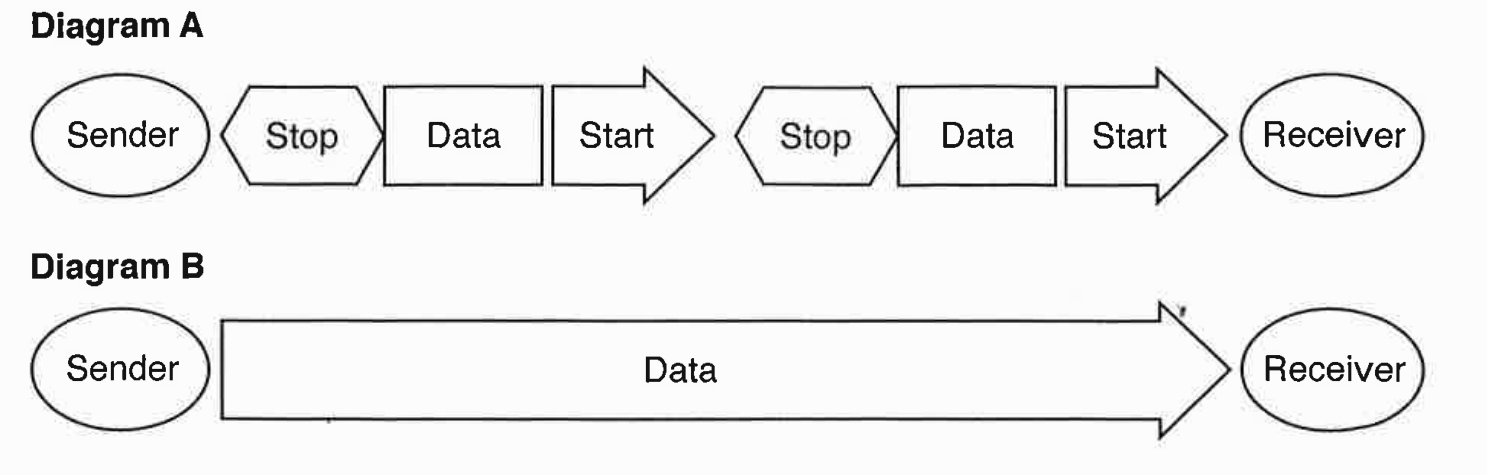
\includegraphics[width=0.5\paperwidth]{C:/Users/Admin/Desktop/Github/question_bank/LyX/static/img/9597-ALVL-2017-P2-Q2-1}
\par\end{center}
\item Explain why asynchronous data transmission affects network performance.\hfill{}
{[}2{]}
\end{enumerate}
\end{enumerate}
An employee works from home on her wireless laptop. The following
diagram shows the configuration of the employee's home network.
\begin{center}
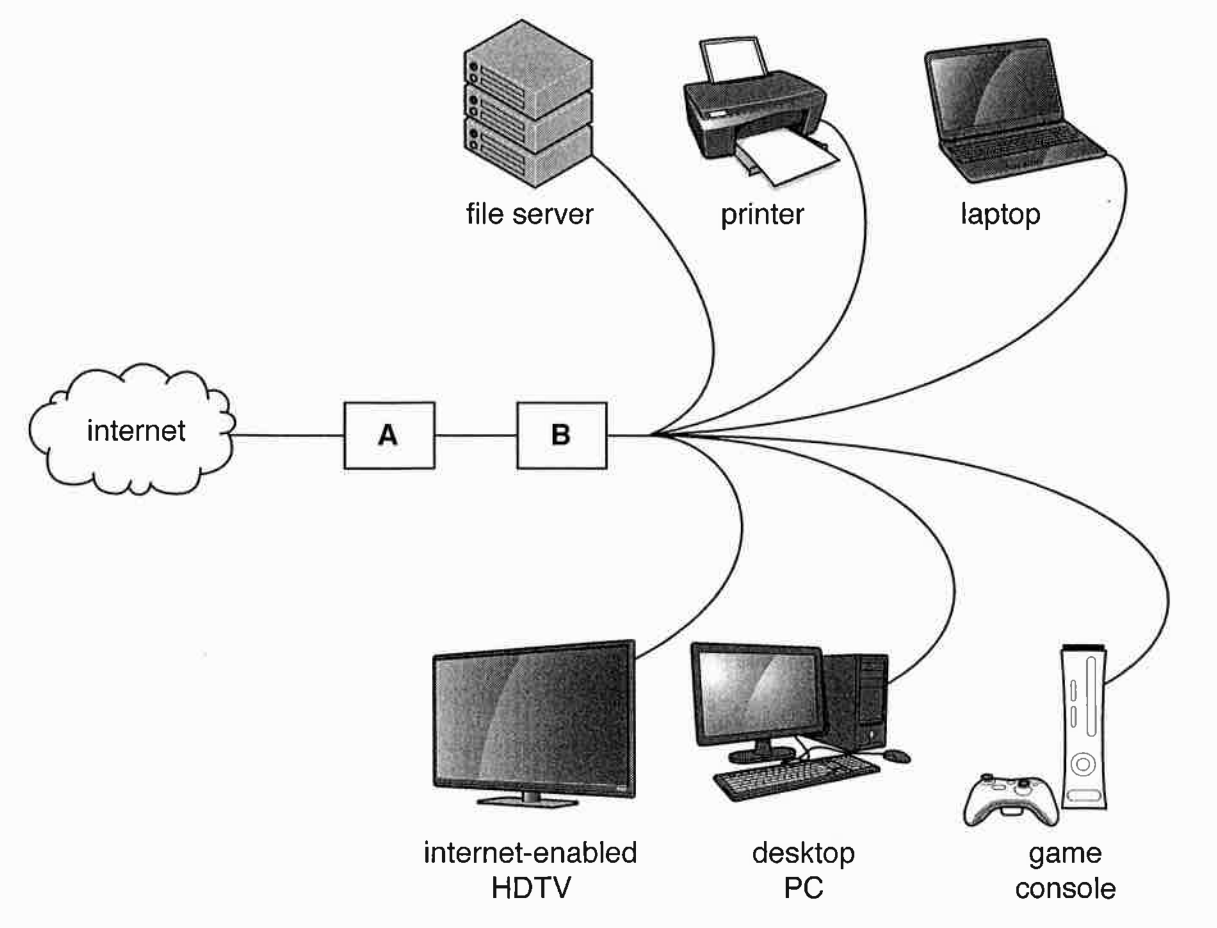
\includegraphics[width=0.5\paperwidth]{C:/Users/Admin/Desktop/Github/question_bank/LyX/static/img/9597-ALVL-2017-P2-Q2-2}
\par\end{center}
\begin{enumerate}
\item[(b)] This network uses both a switch and a router to transfer data. State
which of the pieces of equipment labelled \textbf{A} and \textbf{B}
is the switch. Explain your answer. \hfill{}{[}2{]}
\item[(c)] Describe \textbf{two} features of a router.\hfill{} {[}2{]}
\item[(d)] Describe \textbf{one} advantage and \textbf{one} disadvantage. for
the employee, of working from home.\hfill{} {[}2{]}
\end{enumerate}
{[}SPLIT\_HERE{]}
\item \textbf{{[}ALVL/9597/2017/P2/Q3{]} }
\begin{enumerate}
\item Explain what is meant by an object in object-oriented programming.
.\hfill{}{[}2{]} 
\item {} 
\begin{enumerate}
\item A student is writing a program to represent people in a university.
Tutors, office workers, lecturers and professors are all employed
by the university. A professor is a senior lecturer. The university
educates both undergraduate and graduate students. 

The student\textquoteright s program contains a class with the identifier
\texttt{Person}. Sub-classes share the characteristics of this class. 

Copy and complete the following inheritance diagram by adding sub-classes
\texttt{Professor}, 

\texttt{OfficeWorker}, \texttt{Lecturer}, \texttt{Undergraduate},
\texttt{Staff}, \texttt{Graduate}, \texttt{Student} and \texttt{Tutor}.
\hfill{}{[}2{]} 
\begin{center}
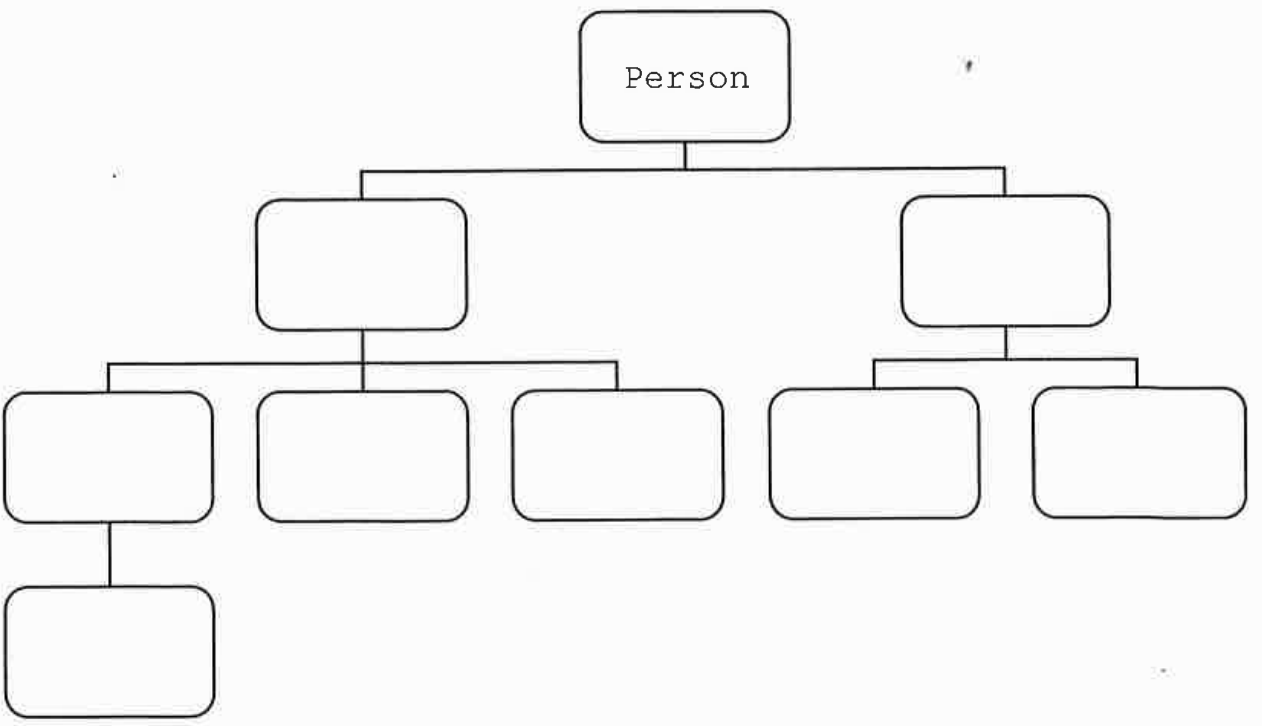
\includegraphics[width=0.5\paperwidth]{C:/Users/Admin/Desktop/Github/question_bank/LyX/static/img/9597-ALVL-2017-P2-Q3}
\par\end{center}
\item Explain why inheritance is an important feature of object-oriented
programming.\hfill{}{[}2{]} 
\end{enumerate}
\item A stack is a data structure that can be implemented in object-oriented
programming. The implementation of a stack requires an integer variable
and an array. 
\begin{enumerate}
\item Describe the purpose of the integer variable in the implementation
of a stack class.\hfill{} {[}1{]}
\item Describe the purpose of the array in the implementation of a stack
class.\hfill{} {[}1{]}
\item Explain how to use the stack data structure to compute the following
expression: 
\noindent \begin{center}
$\left(\text{A}+\text{B}\right)\times\left(\text{C}+\text{D}\right)$\hfill{}
{[}2{]}
\par\end{center}

\end{enumerate}
\end{enumerate}
{[}SPLIT\_HERE{]}
\item \textbf{{[}ALVL/9597/2017/P2/Q4{]} }
\begin{enumerate}
\item A local area network (LAN) can be set up as either client-server or
peer-to-peer. 
\begin{enumerate}
\item State where data are stored on a client-server network. \hfill{}
{[}1{]}
\item State where data are stored on a peer-to-peer network. \hfill{} {[}1{]}
\item Describe \textbf{one} benefit of a client-server network over a peer-to-peer
network. \hfill{} {[}2{]}
\item Describe \textbf{one} drawback of a client-server network compared
to a peer-to-peer network.\hfill{} {[}2{]}
\end{enumerate}
\item A college has five IT rooms. Each room has 20 computers which can
only print to a single printer in the room. At busy times in the year,
there can be up to 100 students printing their coursework at the same
time. \textquoteleft 0

Explain how all these print jobs are controlled and sent to the printer.\hfill{}
{[}2{]}
\item A 30 megabyte file is transferred over a network to a printer in 5
seconds. 

Calculate the transfer rate, in megabits per second, used to transfer
this file. Show all of your working. \hfill{} {[}2{]}
\end{enumerate}
{[}SPLIT\_HERE{]}
\item \textbf{{[}ALVL/9597/2017/P2/Q5{]} }The following grid shows the initial
state of a popular puzzle.
\begin{center}
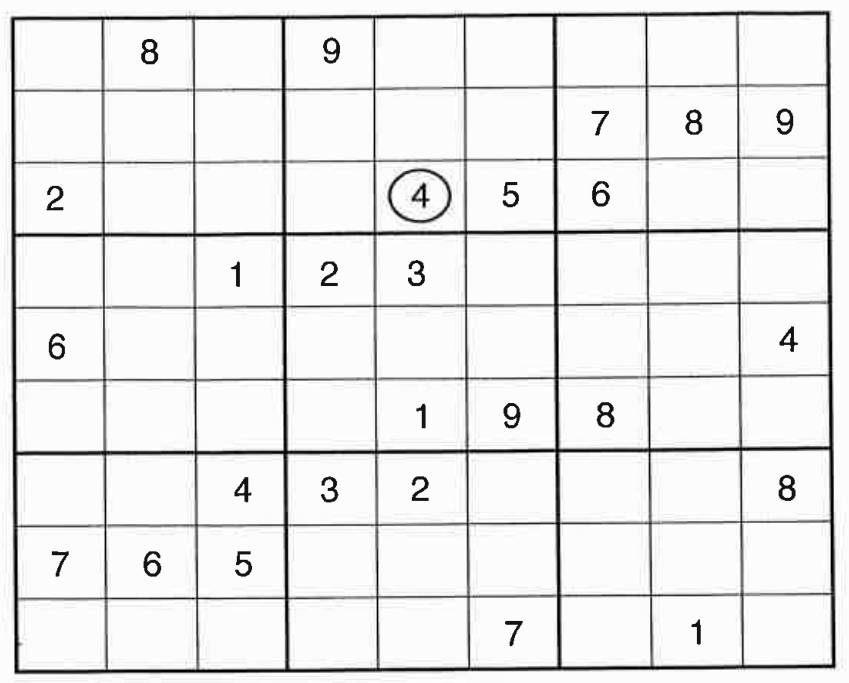
\includegraphics[width=0.5\paperwidth]{C:/Users/Admin/Desktop/Github/question_bank/LyX/static/img/9597-ALVL-2017-P2-Q5}
\par\end{center}

The aim of the puzzle is to fill the whole grid so that every row,
every column and every $3\times3$ mini-grid contains a number between
1 and 9. No number should be repeated in any row, column or 3 x 3
minigrid. 

A software company is creating an online version of the puzzle. A
programmer is asked to create the puzzle software. 
\begin{enumerate}
\item The programmer decides to use a 2D array to store the puzzle.
\begin{enumerate}
\item Copy and complete the following line of pseudocode. 

\texttt{DECLARE Puzzle ARRAY{[}1 : ...., .... : ....{]} OF ......................}
\hfill{}{[}2{]}

The circled value in the diagram above needs to be assigned to the
appropriate array element. 
\item Copy and complete the following line of pseudocode. 

\texttt{Puzzle{[}...., ....{]} <- ...............................}
\hfill{}{[}2{]}
\item Explain why a 2D array is more suitable than a single 1D array to
represent this puzzle. \hfill{}{[}2{]}
\end{enumerate}
\item The puzzle grid can be saved by writing the array \texttt{Puzzle}
to a file. 

Design an algorithm, using pseudocode, to write the array to the file.
\hfill{} {[}5{]}
\item During the testing of the puzzle software, several errors are discovered. 

Describe \textbf{two} debugging techniques that could be used to locate
these errors. \hfill{}{[}4{]}
\end{enumerate}
{[}SPLIT\_HERE{]}
\item \textbf{{[}ALVL/9597/2017/P2/Q6{]} }

A computer company has several offices throughout the country, each
with several salespersons. A record of the sales made by each salesperson
has been set up using a relational database. There is a minimum amount
of \$150 for each sale.

The following tables hold the data. 

\texttt{CUSTOMER (}\texttt{\uline{CustomerID}}\texttt{, CustomerName,
CustomerEmail, CustomerTelephone) }

\texttt{OFFICE (}\texttt{\uline{OfficeID}}\texttt{, Address, Telephone) }

\texttt{SALE (}\texttt{\uline{CustomerID{*}}}\texttt{, }\texttt{\uline{SalesPersonID{*}}}\texttt{,
SaleDate, Amount) }

\texttt{SALESPERSON (}\texttt{\uline{SalesPersonID}}\texttt{, SalespersonName,
OfficeID{*}) }

\textbf{Note:} underline indicates primary key. An asterisk ({*})
indicates a foreign key. 
\begin{enumerate}
\item Draw an Entity-Relationship (E-Fl) diagram to represent the data model.
\hfill{} {[}3{]} 
\item (b) The following is a section of the data dictionary for the data
model. it has three missing entries labelled \textbf{A}, \textbf{B
}and \textbf{C}.
\begin{center}
\begin{tabular}{|l|l|l|c|}
\hline 
\texttt{\textbf{\hspace{0.01\columnwidth}}}\textbf{Table} & \texttt{\textbf{\hspace{0.01\columnwidth}}}\textbf{Field} & \textbf{Data type} & \textbf{Validation}\tabularnewline
\hline 
\texttt{CUSTOMER} & \texttt{CustomerID} & Integer & Unique\tabularnewline
\hline 
\texttt{SALE} & \texttt{CustomerID} & Integer & \textbf{A}\tabularnewline
\hline 
\texttt{SALE} & \texttt{SaleData} & Date & \tabularnewline
\hline 
\texttt{SALE} & \texttt{Amount} & \texttt{\textbf{\hspace{0.01\columnwidth}}}\textbf{B} & \textbf{C}\tabularnewline
\hline 
\end{tabular}
\par\end{center}

State a suitable entry for \textbf{A}, \textbf{B} and \textbf{C}.
\hfill{}{[}3{]} 
\item There is an address field in this database.

Explain why storing the address as a single field is not good database
design. \hfill{}{[}3{]}
\end{enumerate}
Each month, a report is produced to show the sales for each salesperson.
The following is a report for salesperson, B Chin. 
\begin{center}
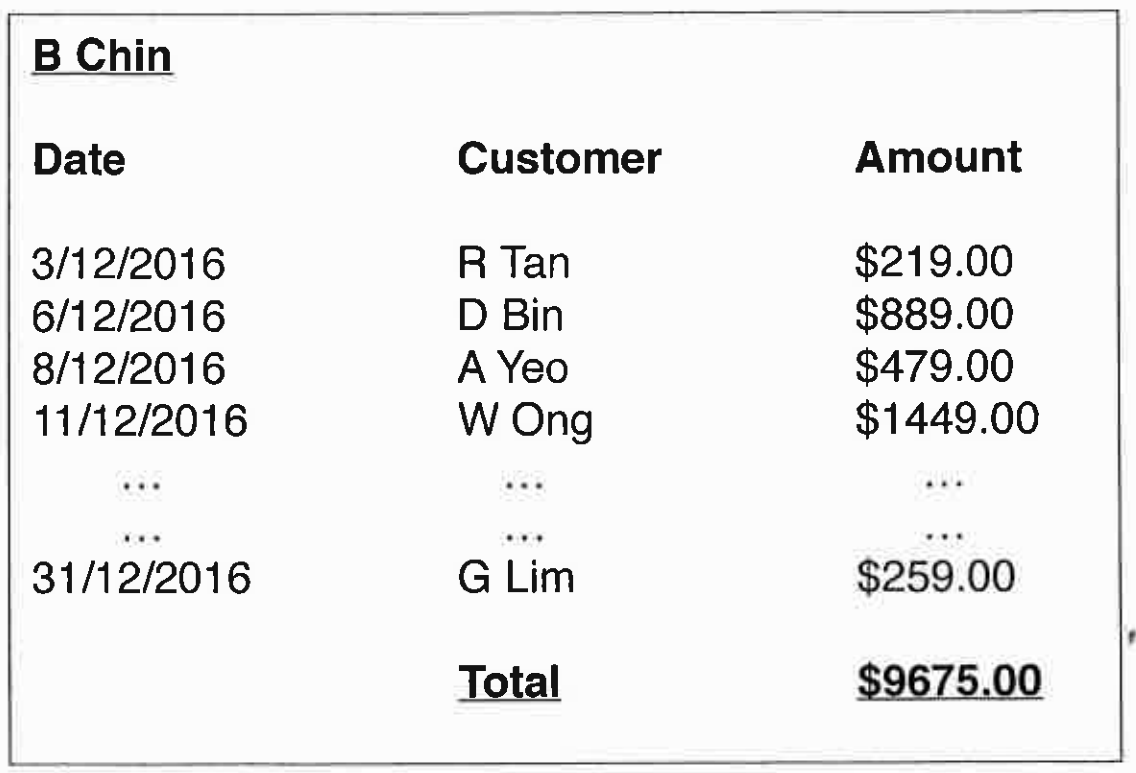
\includegraphics[width=0.5\paperwidth]{C:/Users/Admin/Desktop/Github/question_bank/LyX/static/img/9597-ALVL-2017-P2-Q6}
\par\end{center}
\begin{enumerate}
\item[(d)] {}
\begin{enumerate}
\item To produce the report, the database uses the \texttt{SaleDate} and
\texttt{Amount} fields in the \texttt{SALE} table. 

Name \textbf{four }other fields that the database uses to produce
this report.\hfill{} {[}4{]}
\item State \textbf{two} features of a relational database management system
which would be used to calculate and display the total for this salesperson.\hfill{}
{[}2{]}
\end{enumerate}
\end{enumerate}
{[}SPLIT\_HERE{]}
\end{enumerate}

\end{document}
